\chapter{THE STANDARD MODEL} \label{sm}

The Standard Model (SM) of particle physics is an incredibly successful theory that correctly describes the physics of all known particles and forces that make up the universe, excluding gravity \cite{smconsistency}. The particles of the SM come in two types, fermions and bosons \footnote{Bosons have integer spin.}. Fermions are the spin 1/2 particles and make up the different types of matter. Electrons are a familiar example, and the up and down quarks that make up protons and neutrons are some other examples of fermions. While electrons and the up and down quarks account for nearly all of the matter in our day to day experience there are actually many other fermions. In fact, there are three generations of quarks and leptons \footnote{Leptons are fermions that aren't quarks.} with each generation heavier than the next. The up and down quarks are the first generation of quarks, charmed and strange are the next, and top and bottom are the third generation. For the leptons the electron and electron neutrino are the first generation, the muon and muon neutrino are the second, and the tau and the tau neutrino the third. Each fermion also has a corresponding antiparticle. As an example, the positron is the antiparticle for the electron. 

\begin{figure}[h!]
  \centering
  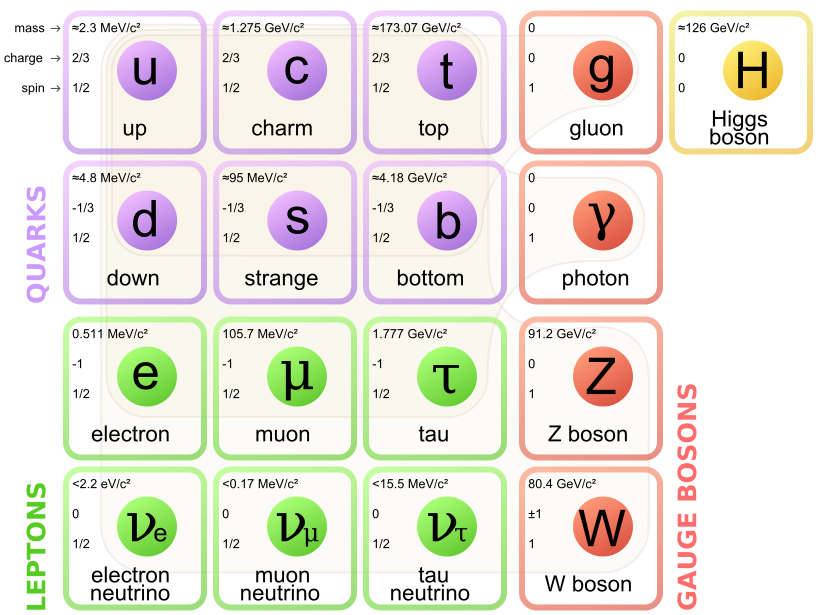
\includegraphics[width=4in]{images/Standard_Model_of_Elementary_Particles.png}
  \caption
   {The Standard Model Particles}
  \label{fig:smtable}
\end{figure}

The universe would be pretty boring if the particles couldn't attract or repel or form more complex objects like atoms, molecules, and even people. Luckily there are forces as well and these forces are described by the spin 1 bosons. The fermions attract and repel by exchanging bosons, which is why the bosons are often called force carriers. Gluons mediate the strong force, photons the electromagnetic force, and the W and Z bosons mediate the weak force. Every force has an associated charge. Just as those particles with electric charge can interact through the electromagnetic force, those with color charge may interact via the strong force, and those with isospin may interact through the weak force. The fundamental forces and particles interact to make the familiar composite objects that surround us in our daily lives. The strong force binds quarks to form protons and neutrons, the Van Der Waals version of the strong force binds the protons and neutrons together to form nuclei, and the electromagnetic force binds electrons and nuclei to form atoms. The size of the composite objects gives an idea of the relative strength of the forces. A proton is ~$10^-15$ meters in size while an atom is ~$10^-10$ meters and a solar system is ~$10^12$ meters. The more tightly bound the stronger the force. In fact the ratio of the strength of the forces is like so 1:$10^-3$:$10^-16$:$10^-41$, strong : electromagnetic : weak :gravitational \footnote{Gravity is just included for perspective. The Standard Model does not describe this force and reconciling gravity with quantum mechanics is an open problem.}. 

Of all the particles predicted by the SM, only the Higgs boson remains to be found. The Higgs boson is the only spin 0 particle of the SM. It is theorized that as the universe cooled from the Big Bang the Higgs field went through a phase transition and settled into a nonzero ground state forming a condensate. And it is the potential energy from the interactions with this ground state that give the massive fundamental particles their mass. With such a large role in the SM, finding this particle or a BSM Higgs has been a huge priority for the CMS collaboration \cite{tdr}. In 2012 a Higgs particle with a mass of 125 GeV was found and to date remains consistent with the Standard Model. However, the properties need to be investigated further before declaring the discovered Higgs the Higgs of the Standard Model. 


%%%%%%%%%%%%%%%%%%%%%%%%%%%%%%%%%%%%%%%%%%%%%%%%%%%%%%%%%%%%%%%%%%%%%%%%%%%

\section{Quantum Field Theory}

The mathematical framework used to describe the physics of the SM as well as other Beyond Standard Model (BSM) field theories is called Quantum Field Theory (QFT). QFT enables the predictions of measurable quantities, namely the probabilities for different sets of particles to come out of a specific collision or for a single particle to decay into different sets of particles. These probabilities are encompassed in the cross sections and branching fractions. For example, the theory of the SM predicts the cross section for two protons colliding and making a Higgs. As another example, the SM also predicts the branching fraction for a Z boson decaying to two muons. These probabilities can be measured simply by colliding particles and counting the outcomes which in turn means that the theory can be tested. In fact, any QFT model can be tested in this manner. There are other commonly measured properties as well like the lifetime, spin, and mass of different particles.  

\subsection{What is a Particle?}

Consider an observer in a frame x with particle p and an observer in another frame x'. If the observer in x' can't identify particle p then it doesn't make sense to call p a particle. More concretely, consider a world where in frame x an observer sees a neatly stacked deck of cards, but in x' the observer sees the cards scattered all over the place. Calling the deck of cards a particle doesn't really make sense. On the other hand, both parties can still agree on the individual cards which kept the same suit and value. These are conserved quantities. If the two observers get together later and compare notes they can see what happened to each card upon transforming from x to x' and work out a set of rules. The king of hearts may do one thing and the 10 of clubs another. They can then add the different forces into play repeat the process and compare again. Figuring this all out determines the laws of physics for the fundamental pieces called particles.       

This idea leads to Wigner's view: a particle is an object with conserved quantities that observers can agree on between frames. In our universe these labels are the mass, charge, spin, color, and isospin. And because different observers can agree on these quantities they can compare notes and work out the laws of physics for the different types of particles. All that remains is to work out laws that people in different frames can confirm. 

\subsection{The Lagrangian Formalism}

This section covers the Lagrangian formalism that allows physicists to describe the evolution of a physical system over time. A simple example of the free Newtonian particle is given and different symmetries are observed. The most important of which is the fact that the laws of physics are indistinguishable in different inertial frames. Using this as a postulate along with the requirement that the speed of light remain constant in all frames of reference, QFT will then be built. 

The goal of physics is to describe how a physical system evolves over time. The evolution over time is usually given by some differential equation describing the state the system will take in the next interval of time given the current time. Moving from state to state from one interval of time to the next, the system traces out some path in space and time or some other more abstract space of possible states. As it turns out nature tries to minimize the difference between the energy spent \footnote{Spent here just means used as kinetic energy.} and the energy available to spend and it minimizes the action S. In the equation below, L is the Lagrangian, T is the kinetic energy and U is the potential energy.     
\begin{equation}
S = \int L dt = \int T - U dt
\end{equation}

At an extremum of S, $\delta S$ = 0 since S must go down and back up or vice versa. So to get the equations of motion just vary the parameters of L and solve for the values that yield zero change in the action.

\begin{equation}
\delta S = \int L(z_1 + dz_1, z_2+dz_2, ...)dt - \int L(z_1, z_2, ...)dt 
\end{equation}

This will yield the Euler-Lagrange equations, describing how the parameters z evolve over time. The z's may be the position and velocity, or the quantum fields, or the temperature and volume or some other set of parameters that describe the system. The Lagrangian for a Newtonian free particle in one dimension is pretty simple and gets the point across. 

\begin{equation}
S = \frac{1}{2} \int m\dot{x}^2 dt
\end{equation}

If the action is at an extremum, perturbing the path x(t) by adding the infinitesimal $\epsilon$(t) leaves the action unchanged.

\begin{equation}
S' = \frac{1}{2} \int m(\dot{x} + \dot{\epsilon})^2 dt = \frac{1}{2} \int m(\dot{x}^2 + 2\dot{x}\dot{\epsilon} + \dot{\epsilon}^2) dt =  
\frac{1}{2} \int m(\dot{x}^2 + 2\dot{x}d\dot{x}) dt 
\end{equation}

\begin{equation}
\delta S = S' - S = 0 = \frac{1}{2} \int m(\dot{x}^2 + 2\dot{x}\dot{\epsilon}) dt - \frac{1}{2} \int m\dot{x}^2 dt = \int m\dot{x}\dot{\epsilon} dt
\end{equation}

Since x(t) is fixed at the boundaries of the integral, $\epsilon$ must be zero at $t_o$ and $t_f$, so integrating by parts yields the following equation. 

\begin{equation}
\delta S = 0 = \epsilon(t_f) \dot{x}(t_f)  - \epsilon(t_o) \dot{x}(t_o) + \int m\ddot{x} \epsilon dt  = 
0\dot{x}(t_f)  - 0\dot{x}(t_o) + \int m\ddot{x} \epsilon dt = \int m\ddot{x} \epsilon dt
\end{equation}

And this equation must be zero for any infinitesimal deviation $\epsilon$.

\begin{equation}
\delta S = 0 \rightarrow m\ddot{x} = 0
\end{equation}

So a free particle keeps the same velocity over time. Note that a Newtonian boost by constant velocity $v \rightarrow v' = v + u$ \footnote{Renaming $\dot{x}$ as v.} leaves the equations of motion consistent. In the unprimed frame the particle has velocity v with 0 acceleration. In the primed frame the particle has velocity v + u with 0 acceleration. Both observers see the particle act as if there are zero forces.

\begin{equation}
S = \frac{1}{2} \int m(v + u)^2 dt  =  \frac{1}{2} \int m(v')^2 dt \rightarrow \delta S = 0 \rightarrow m\frac{d}{dt}(v+u) = m\frac{d}{dt}(v') = 0 
\end{equation}

If u is not constant but a function of time u(t) then the equations of motion do not describe the same time evolution.

\begin{equation}
m\frac{d}{dt}(v+u) = m\dot{v} + m\dot{u} = 0 \rightarrow \dot{v} = -\dot{u}
\end{equation}

In the case where u(t) depends upon time, the difference between the primed and unprimed frames' equations of motion is then $\delta F$.

\begin{equation}
\delta F = m\frac{d}{dt}(v+u) - m\frac{dv}{dt} = m\dot{v} + m\dot{u} - m\dot{v} = m\dot{u}
\end{equation}

In the unprimed frame, the particle identified by the mass moves with constant velocity, $\dot{v} = 0$. The observer in the primed frame looks at the particle with the same mass and sees it change velocity given by the equation $\dot{v} = -\dot{u}$. As an example, set v and $u, \dot{u}$ to zero for all times before t=0, and let $u, \dot{u}$ turn on after time 0. Both observers will agree that the particle is stationary up until time 0. After which, the observer in the primed frame will see the particle accelerate in strange ways. Meanwhile, the unprimed frame will continue to observe a stationary particle. 

In general, every inertial frame finds $\delta F = 0$ and every accelerating frame finds an extra force $\delta F$ unique to its acceleration. In this way no observer in an inertial frame can perform an experiment and determine which inertial frame he or she is in. On the other hand, each accelerating frame is identified by its $\delta F$.  In every inertial frame a ball released at rest remains at rest. In an accelerating frame the ball will accelerate according to the motion of the frame $\delta F$. Since the laws of physics remain the same boosting between inertial frames this is a symmetry of physics. Of course this example is Newtonian and the correct way to boost is given by the Lorentz transformation from Special Relativity, but this gets the point across.

Since the fundamental forces depend only on the distance from the charge and not the direction, rotations are also a symmetry. This can be seen by looking at the Lagrangian. 

\begin{equation}
L = \frac{1}{2} m\dot{\vec{x}}^2 - U((\vec{x} - \vec{x'})^2)
\end{equation}

Rotations leave dot products and consequently the magnitude of vectors unchanged so the Lagrangian is invariant under this transformation. Naturally if the Lagrangian is invariant the equations of motion will be as well.

\begin{equation}
m\frac{d\vec{v}}{dt} = \vec{\nabla} U
\end{equation}

In the equations of motion above, both sides are vectors and vectors transform the same way under rotations so the equations of motion are invariant. Note that in the case of rotations both the Lagrangian and the equations of motion are invariant. While for Newtonian boosts only the equations of motion were invariant. This is due to the fact that Newtonian mechanics is the low velocity limit of relativistic mechanics. In the theory of Special Relativity the action for a massive free particle is written like so.

\begin{equation}
S = \int \frac{m}{2}u^{\mu}u_{\mu}d\tau
\end{equation}

\subsection{QFT From Symmetry}

\subsection{Perturbation Theory}

\subsection{Feynman Rules}

\begin{figure}[h!]
  \centering
  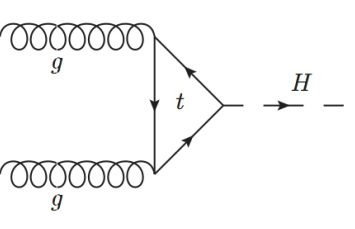
\includegraphics[width=1.5in]{images/ggf.png}
  \caption
   {The Feynman diagram for two gluons fusing into a Higgs. There are three vertices and this is a third order diagram. Two vertices involve the strong force and one vertex involves the Higgs coupling. The matrix element for this diagram would have two factors of the strong force coupling and one factor for the Higgs coupling which involves the mass of the top quark.}
  \label{fig:feynggf}
\end{figure}

%%%%%%%%%%%%%%%%%%%%%%%%%%%%%%%%%%%%%%%%%%%%%%%%%%%%%%%%%%%%%%%%%%%%%%%%%%%
\section{The Standard Model Higgs}


%%%%%%%%%%%%%%%%%%%%%%%%%%%%%%%%%%%%%%%%%%%%%%%%%%%%%%%%%%%%%%%%%%%%%%%%%%%
\subsection{SM Higgs Production and Decay Modes}

The SM Higgs can be created in a variety of ways. Some of these cross sections are shown below for 14 TeV collisions. The production cross sections are functions of the mass of the Higgs as well as the energy of the collisons. For a given collision energy the cross sections decrease as the Higgs mass increases: there are fewer kinematic possibilities for a heavier particle since more of the energy was used to create the particle. For a given mass, say 125 GeV, the cross section grows with collision energy. This constrasts with cross sections involving collisions of fundamental particles, e.g. electron antielectron collisions. This is an artifact of the fact that the LHC collides protons together. 

\begin{figure}[h!]
  \centering
  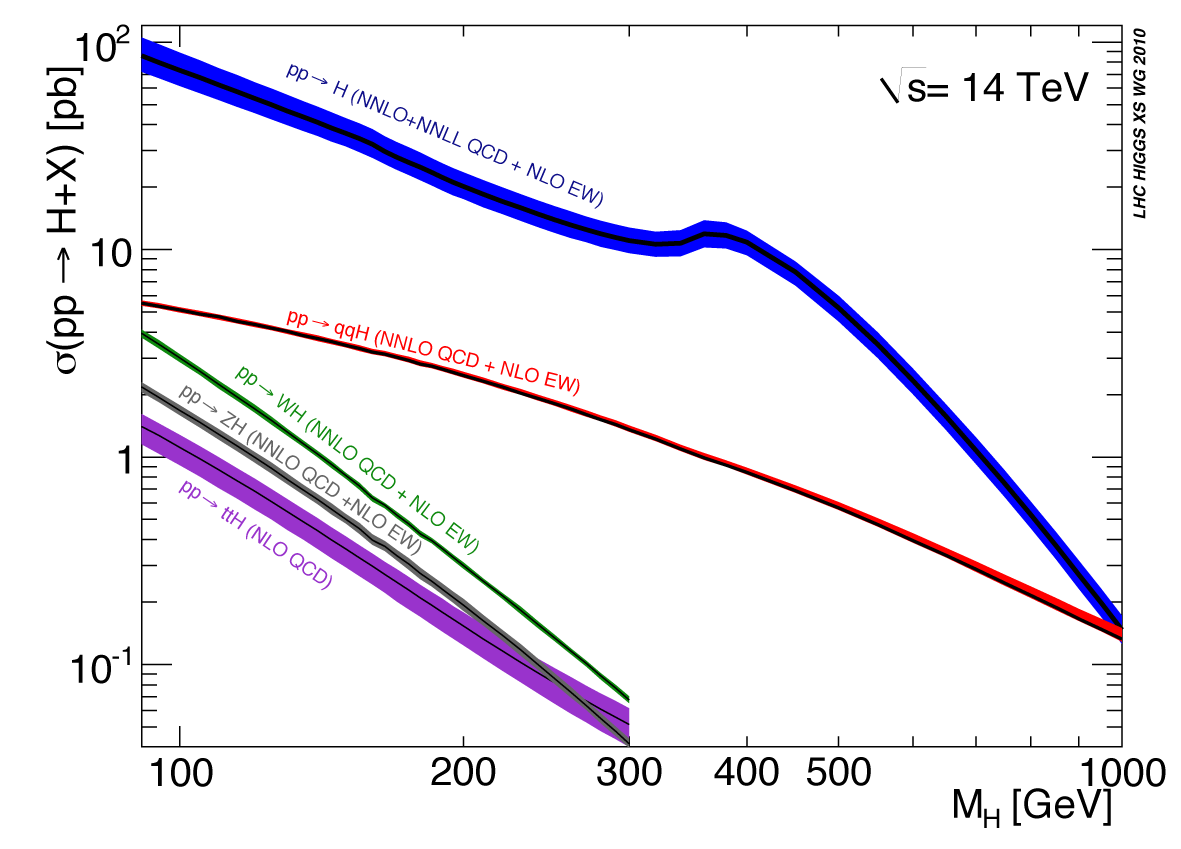
\includegraphics[width=5in]{images/14TeV_higgs_cross_sections.png}
  \caption
   {The highest production mode cross sections for the SM Higgs \cite{crossbranchplots}}
  \label{fig:hprodcross}
\end{figure}

Protons behave like a collection of an infinite number of quark-antiquarks, an infinite number of gluons, and the usual uud. The total momentum of the proton is divided up amongst them with lots of particles having little of the total momentum. The actual scattering events are between these more fundamental particles. The larger the total energy the smaller the fraction of energy needed to make a Higgs and since there are more particles with a lower fraction, this results in a growth of the cross section with collision energy. 

The SM Higgs is unstable and decays with a width of $\sim 5 MeV$ at 125 GeV. The probability of each decay changes depending upon the mass of the Higgs. In general the Higgs couples more strongly to particles with higher mass making the decays to heavier particles more likely.  

\begin{figure}[h!]
  \centering
  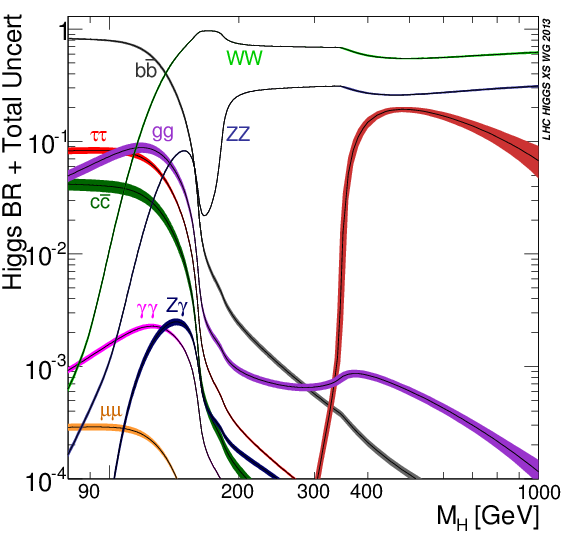
\includegraphics[width=3in]{images/Higgs_BR.png}
  \begin{tabular}{ |l|l| }
    \hline
    \multicolumn{2}{|c|}{Higgs Branching Ratios} \\
    \hline
    ${\rm b\bar{b}}$ & 0.57 \\
    WW & 0.22\\
    gg & 0.085 \\
    ${\rm \tau\tau}$ & 0.065 \\
    ZZ & 0.027 \\
    ${\rm c\bar{c}}$ & 0.027 \\
    ${\rm \gamma\gamma}$ & 0.0023 \\
    ${\rm Z}\gamma$ & 0.0016 \\
    ${\rm \mu^{+}\mu^{-}}$ & 0.00022 \\
    \hline
  \end{tabular} 
  \caption
{The graphic on the top left presents the SM Higgs branching fractions as functions of mass while the table on the bottom right displays the branching fractions for a 125 GeV SM Higgs \cite{crossbranchplots}.}
  \label{fig:hbranch}
\end{figure}

The muon has the lowest mass -- excluding the photon and gluon -- of the particles in Figure ~\ref{fig:hbranch} and consequently H$\rightarrow \mu^{+}\mu^{-}$ has the lowest branching fraction in the set. \footnote{The Higgs also couples to the electron and the first generation quarks but the masses are so light that CMS does not expect to see the SM Higgs in those modes.} The gluons and photons are massless and do not couple to the Higgs at leading order. These massless vector bosons interact with the Higgs through a loop of top quarks. The extremely heavy mass of the top quark, about 173 GeV, balances the fact that the loop production is a higher order mechanism.  
\begin{figure}[h!]
  \centering
  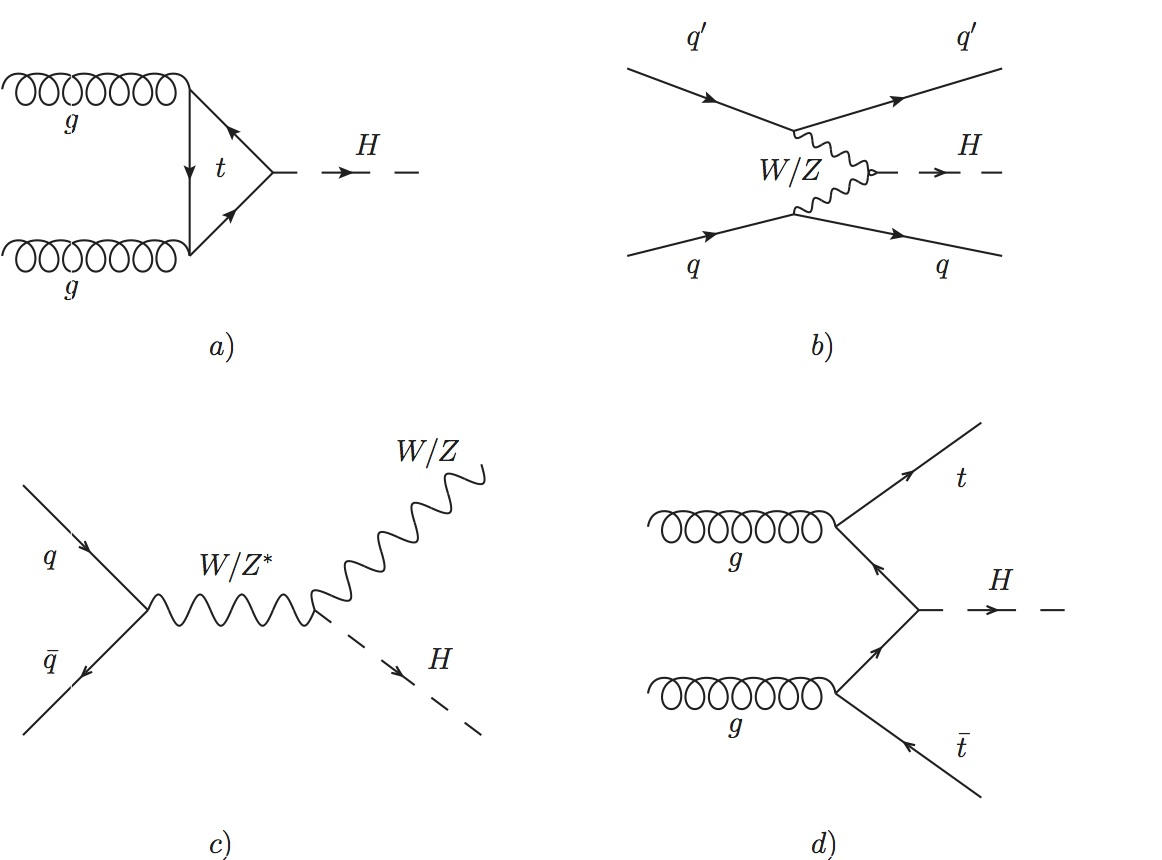
\includegraphics[width=4in]{images/higgs_production_modes.png}
  \caption
   {The SM production modes with the highest cross sections. a) Gluon Gluon Fusion (GF) b) Vector Boson Fusion (VBF) c) Associated Production with a Vector Boson (VH) d) ${\rm t\bar{t}}$H}
  \label{fig:hfeynprod}
\end{figure}

The Higgs to massless vector boson coupling via the top loop is seen in the GF Feynman diagram in Figure ~\ref{fig:hfeynprod}. At ${\rm M_{h} = 125}$ GeV, ${\rm \sqrt{s} =}$ 13 TeV, the GF channel comprises 87\% of the total Higgs production cross section, VBF 7\%, VH 4\%, and ${\rm t\bar{t}}$H 1\% \cite{crossbranchplots}. Besides ${\rm t\bar{t}}$H, the process q + $\bar{q} \rightarrow$ H isn't considered due to its low cross section. The low masses of the other quarks suppress the process. 

Quark gluon (qg) scattering is a major background for the Higgs to two jets decays since the process closely resembles GF in this mode.   

\begin{figure}[h!]
  \centering
  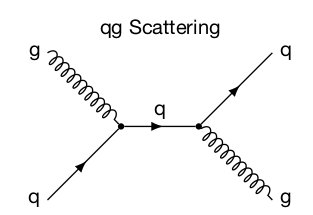
\includegraphics[width=2in]{images/qg_scattering.png}
  \caption
   {Quark gluon scattering creates many two jet events. This background looks very similar to GF when the Higgs decays to two jets. The colliding protons are made of quarks and gluons so this process is extremely common.}
  \label{fig:feynqg}
\end{figure}

